\section{Phase Estimation With Neural Networks}
We try to use a neural network to decide the phase of a given signal segment. We decided to use the following features: AR coefficients, Shannon entropy estimate, percentile frequencies ($f_{25}$, $f_{50}$, $f_{75}$ and $f_{90}$) and the ratio between each of them, variance, spectral magnitude and kurtosis. These features change for each recording, bu the difference between inspiration and expiration doesn't change, so we used z-score before giving these features to neural network. A visual description of estimating the period is given in Figure \ref{fig:estimate_period}. We are looking at the ratio of blue function to the red line at the end.

\subsection{Description of Neural Networks} 
A neural network is a function with many inputs and a single output. Formulation and development of neural networks are inspired from biological nervous system. Input values of a neural network is processed by dozens of interconnected functions, and these functions are called "neuron"s. A neuron can be thought as a function with multiple outputs and a single output. A neuron's output is determined by the activation function \cite{neural-networks}.
\subsubsection{Neuron}
Mathematical expression of a neuron's activation function is given in \eqref{neuron_equation}. Here $\beta$ is the activation function. Activation function may be in several different forms. It is selected based on the application where the neural network is used and the distribution of input values. Activation functions are generally selected or constructed in a way that they are easily differentiable. Some of popular activation functions are given in  figure \ref{fig:activation_fncs}. 
\begin{equation} \label{neuron_equation}
y = \beta(\sum_{i=1}^{N}(w_ix_i))
\end{equation}
\begin{figure}[h] \label{neuron}
	\centering
\tikzstyle{inputNode}=[draw,circle,minimum size=10pt,inner sep=0pt]
\tikzstyle{stateTransition}=[->, thick]
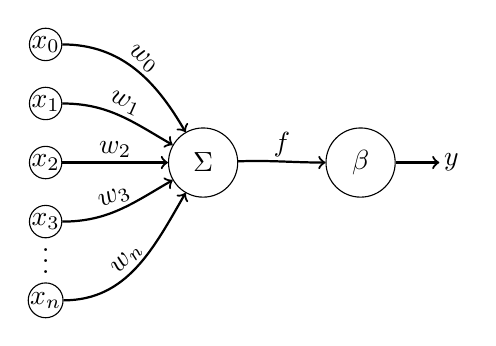
\begin{tikzpicture}
\node[draw,circle,minimum size=25pt,inner sep=0pt] (x) at (0,0) {$\Sigma$};
\node[draw,circle,minimum size=25pt,inner sep=0pt] (y) at (2,0) {$\beta$};

\node[inputNode] (x0) at (-2, 1.5) {$\tiny x_0$};
\node[inputNode] (x1) at (-2, 0.75) {$\tiny x_1$};
\node[inputNode] (x2) at (-2, 0) {$\tiny x_2$};
\node[inputNode] (x3) at (-2, -0.75) {$\tiny x_3$};
\node[inputNode] (xn) at (-2, -1.75) {$\tiny x_n$};

\draw[stateTransition] (x0) to[out=0,in=120] node [midway, sloped, above=-2] {$w_0$} (x);
\draw[stateTransition] (x1) to[out=0,in=150] node [midway, sloped, above=-2] {$w_1$} (x);
\draw[stateTransition] (x2) to[out=0,in=180] node [midway, sloped, above=-2] {$w_2$} (x);
\draw[stateTransition] (x3) to[out=0,in=210] node [midway, sloped, above=-2] {$w_3$} (x);
\draw[stateTransition] (xn) to[out=0,in=240] node [midway, sloped, above=-2] {$w_n$} (x);
\node (dots) at (-2, -1.15) {$\vdots$};
\draw[stateTransition] (x) to[out=2,in=180] node [midway, above=-2] {$f$} (y);
\draw[stateTransition] (y) -- (3,0) node [right,right=-2] {$y$};;
\end{tikzpicture}
\caption{Diagram of A Neuron}
\end{figure}
\begin{figure}
	\begin{center}
		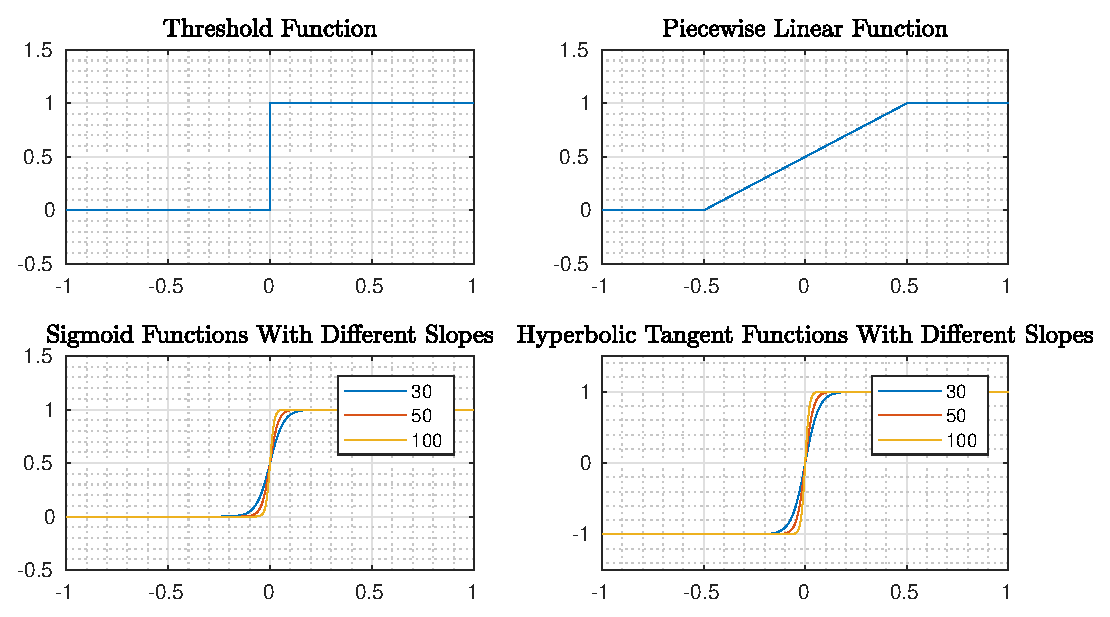
\includegraphics[width=\textwidth]{figures/several_activations.eps}
		\caption{Some Activation Functions}
		\label{fig:activation_fncs}
	\end{center}
\end{figure}
\subsubsection{Layers In Neural Networks}
There are three different layers in neural networks, input layer, output layer and hidden layers. Input and output layers are where the input values are received and output values are given out respectively. Hidden layers are where the information from input layer or previous hidden layer is processed. Hidden layers may have arbitrary number of neurons and there may be any number of hidden layers in a neural network.
\def\layersep{2.5cm}
\begin{figure}[h]
	\centering
	
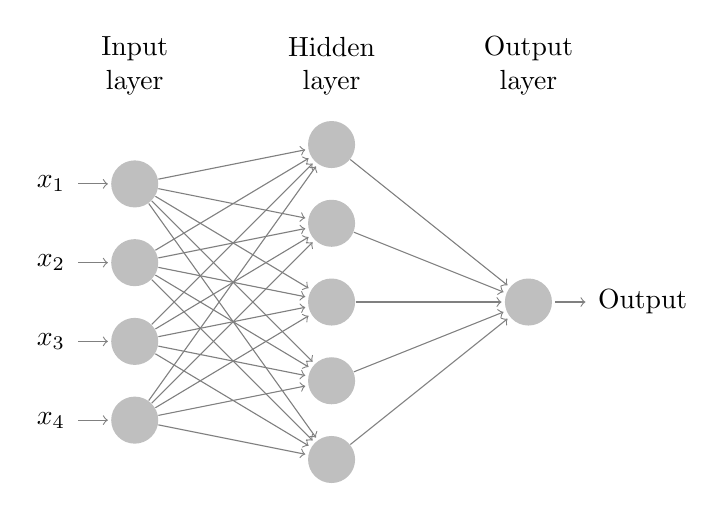
\begin{tikzpicture}[shorten >=1pt,->,draw=black!50, node distance=\layersep]
\tikzstyle{every pin edge}=[<-,shorten <=1pt]
\tikzstyle{neuron}=[circle,fill=black!25,minimum size=17pt,inner sep=0pt]
\tikzstyle{input neuron}=[neuron];
\tikzstyle{output neuron}=[neuron];
\tikzstyle{hidden neuron}=[neuron];
\tikzstyle{annot} = [text width=4em, text centered]

% Draw the input layer nodes
\foreach \name / \y in {1,...,4}
% This is the same as writing \foreach \name / \y in {1/1,2/2,3/3,4/4}
\node[input neuron, pin=left:$x_\y$] (I-\name) at (0,-\y) {};

% Draw the hidden layer nodes
\foreach \name / \y in {1,...,5}
\path[yshift=0.5cm]
node[hidden neuron] (H-\name) at (\layersep,-\y cm) {};

% Draw the output layer node
\node[output neuron,pin={[pin edge={->}]right:Output}, right of=H-3] (O) {};

% Connect every node in the input layer with every node in the
% hidden layer.
\foreach \source in {1,...,4}
\foreach \dest in {1,...,5}
\path (I-\source) edge (H-\dest);

% Connect every node in the hidden layer with the output layer
\foreach \source in {1,...,5}
\path (H-\source) edge (O);

% Annotate the layers
\node[annot,above of=H-1, node distance=1cm] (hl) {Hidden layer};
\node[annot,left of=hl] {Input layer};
\node[annot,right of=hl] {Output layer};
\end{tikzpicture}
\caption{A Neural Network With One Hidden Layer}
\end{figure}

\subsubsection{Learning Process In Neural Networks}
Learning is the primary property of neural networks; it enables a neural network to improve its performance. \par 
The learning processes can be divided into three categories with respect to the learning paradigms. These categories are supervised, reinforcement and unsupervised learning. In supervised learning, the desired output is available so the error is known in the learning process. In reinforcement learning there is a performance measure which is being tried to be maximized. In unsupervised learning, neither desired output nor performance measure is available. We will use  supervised learning since the correct phases are known to us. \par
Learning methods can be divided into four sections, error-correction learning, memory based learning, Hebbian learning, competitive learning and Boltzmann learning. We will use error-correction learning and try to minimize the total error measure by adjusting the synaptic weights.
\subsection{Features}
In this section, we will look at the features that will be used in neural network approach. Each feature is found for all the sounds. However while looking at features, one can see that the patterns don't change however the range of values change. To overcome this issue each feature series from each sound gets normalized by  using z-score. Z-score is the measure which gives how much distance a random sample has to its source mean. The formula for z-score is given in \eqref{eq:z-score}
\begin{equation}\label{eq:z-score}
z_i = \frac{x_i - \hat{\mu}_X}{\hat{\sigma}_X}
\end{equation} \par
We also used the Kullback-Leibler (KL) divergence to quantify how much the distributions for inspiration and expiration differ from each other for each feature. KL-divergence is a definition from information theory and it gives a distance between probability distributions. The formula for KL-divergence is given in \eqref{eq:kl-divergence} \cite{info-theory}.
\begin{equation}\label{eq:kl-divergence}
D_{KL}(p(x)||q(x)) = \sum_{x \in X}p(x)\log\frac{q(x)}{p(x)}
\end{equation} 
\subsubsection{AR Coefficients}
When we modeled the respiratory sounds as AR processes and solve for the AR coefficients, we saw that estimated AR coefficients are behaving differently for inspiration and expiration. To give an example, for the case of first AR coefficient it seems as the coefficients are attenuated for expiration phases. So we decided to use  AR coefficients as a feature to the neural network. A detailed explanation about AR models and methods to estimate AR coefficients is given in Section \ref{chp:airflow_curve_estimation}. \\ Distributions of AR coefficients during inspiration and expiration for third channel is given in Figure \ref{fig:arall_ins_exp}
\begin{figure}[h!]
	\begin{center}
		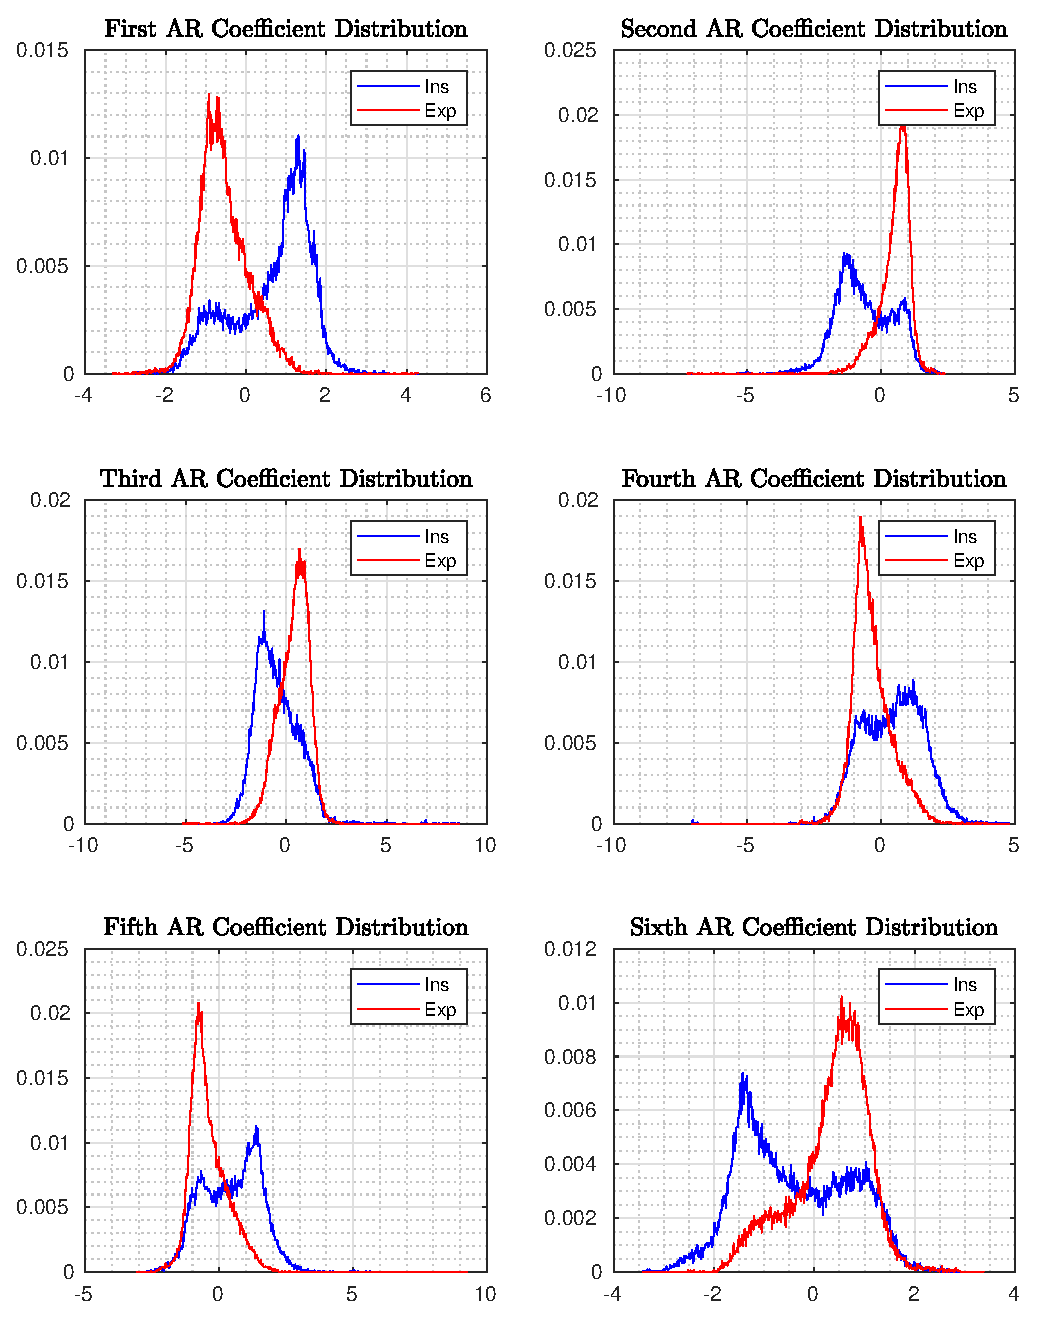
\includegraphics[width=\textwidth]{figures/arall_ins_exp.eps}
		\caption{Distribution of AR Coefficients For Inspiration and Expiration}
		\label{fig:arall_ins_exp}
	\end{center}
\end{figure}
\subsubsection{Shannon Entropy Estimate}
Entropy is a measure which gives information about the complexity of the samples collected. As the randomness of the samples increases entropy increases too. The formula to calculate entropy is given in \eqref{eq:entropy} \cite{info-theory}.  In general we have a wider range for signal values in inspiration, so we expect entropy to be greater for the segments belonging to inspiration. \\ Distributions of Shannon's entropy estimates during inspiration and expiration for third channel is given in Figure \ref{fig:entropy_ins_exp}
\begin{equation}\label{eq:entropy}
	H(X) = - \sum_{x \in X}p(x)\log(x)
\end{equation}
\begin{figure}
	\begin{center}
		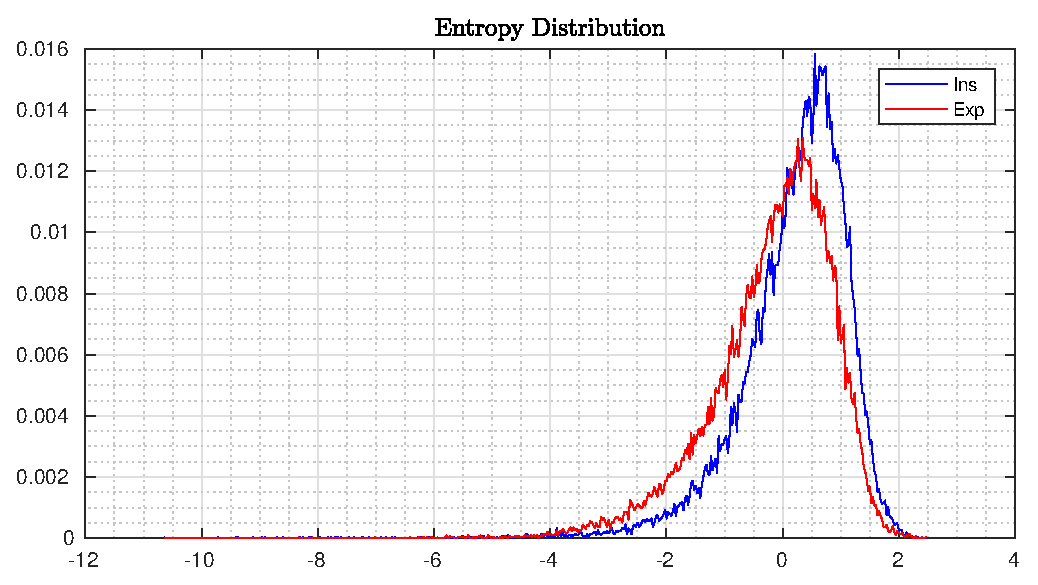
\includegraphics[width=\textwidth]{figures/entropy_ins_exp.eps}
		\caption{Distribution of Shannon Entropy Estimate For Inspiration and Expiration}
		\label{fig:entropy_ins_exp}
	\end{center}
\end{figure} 
\subsubsection{Percentile Frequencies}
A percentile frequency is defined together with the percent. It is the frequency until which the cumulative sum of power spectral density is equal to the defined percent of total power. In order to calculate them, we first estimate the power spectral density according to the formula in Percentile frequencies and their relations are measures which are widely used in respiratory signal analysis \cite{sergul, comparison-ar-based}. Since the expiration and inspiration phases have different time-frequency content, percentile frequencies may be used as input to classifier neural network. Definition of a percentile frequency is given in \eqref{percentf} \\ Distributions of percentile frequencies and their ratios between each other during inspiration and expiration for third channel is given in Figure \ref{fig:percent_ins_exp}.
\begin{align}
	X(f) = \int_{-\infty}^{\infty}x(t)e^{-2{\i}ft\pi}dt \label{ft} \\
	P_{XX}(f) = X(f)^2 \label{psd}\\
	f_{y} = \underset{x}\argmin \frac{\int_{0}^{x} P_{XX}(f) df}{\int_{0}^{\infty} P_{XX}(f) df}   > \frac{y}{100} \label{percentf}
\end{align}
\begin{figure}
	\begin{center}
		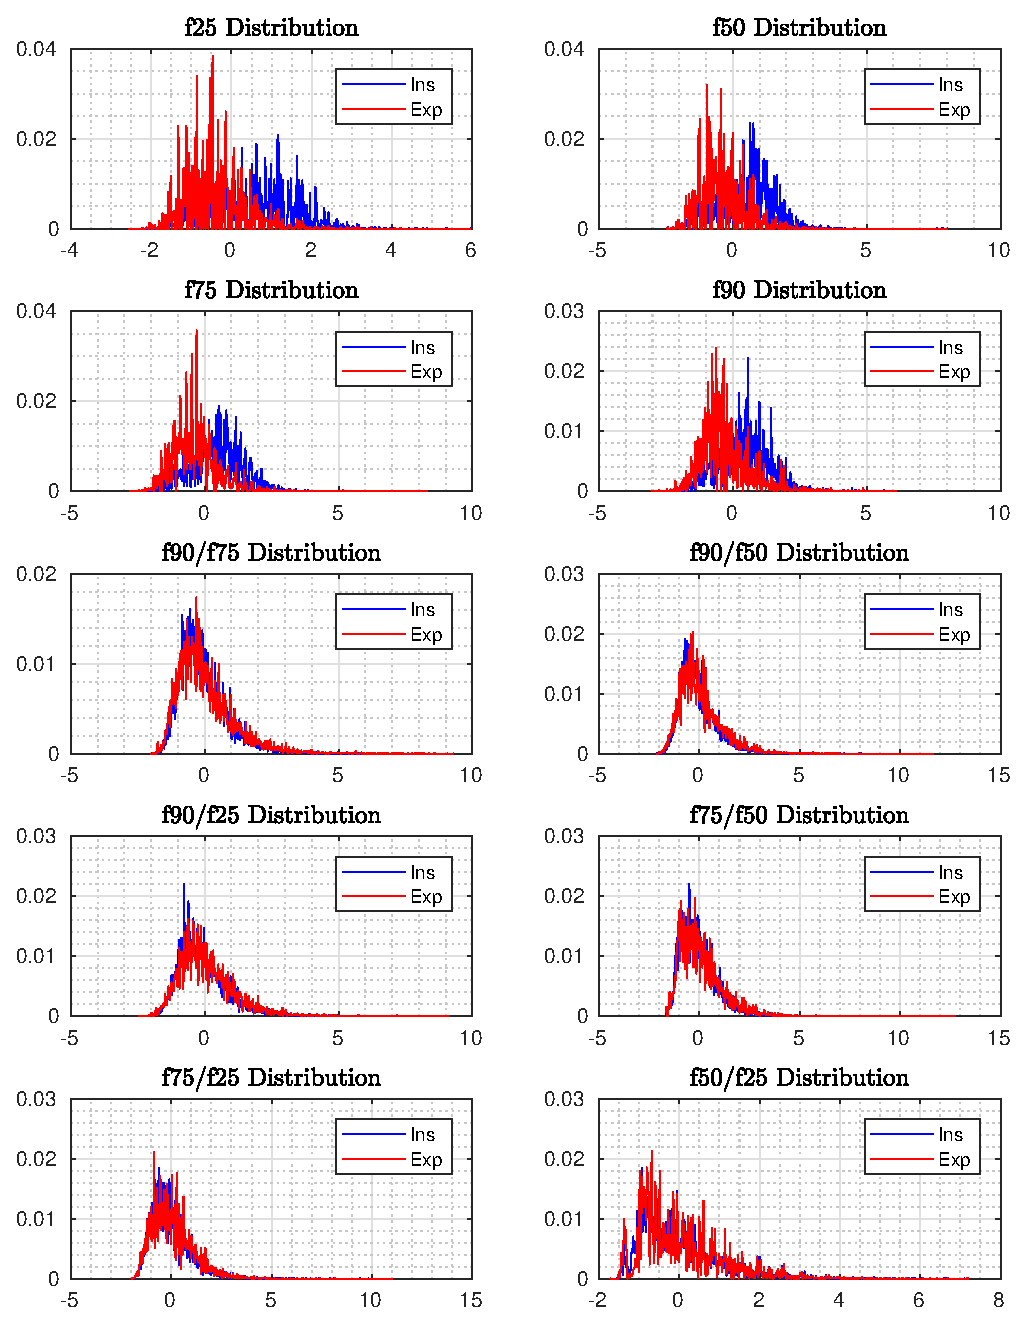
\includegraphics[width=\textwidth]{figures/percent_ins_exp.eps}
		\caption{Distribution of Percentile Frequency Measures For Inspiration and Expiration}
		\label{fig:percent_ins_exp}
	\end{center}
\end{figure}
\subsubsection{Variance}
Variance corresponds to power and observations show that power for different respiratory phases differs. So we decided to use variance as a supportive feature. Sample variance is calculated as in \eqref{sample_variance}. \\ Distributions of variance of windows during inspiration and expiration for third channel is given in Figure \ref{fig:percent_ins_exp}.
\begin{align}
	\hat{\mu}_{X} = \frac{\sum_{x \in X}x}{|X|} \label{sample_mean} \\
	\hat{\sigma}_{X}^2 = \frac{\sum_{x \in X}(x-\hat{\mu}_X)^2}{|X|-1}\label{sample_variance}
\end{align}
\begin{figure}
	\begin{center}
		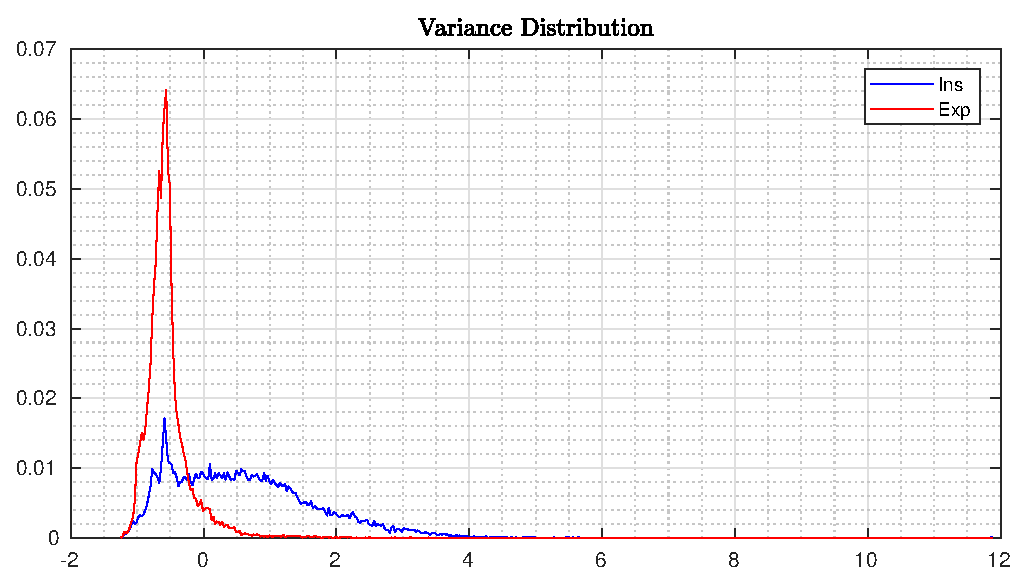
\includegraphics[width=\textwidth]{figures/variance_ins_exp.eps}
		\caption{Distribution of Variance For Inspiration and Expiration}
		\label{fig:variance_ins_exp}
	\end{center}
\end{figure}
\subsubsection{Spectral Magnitude}
The magnitudes of several frequency bands are calculated for each segment using FFT. We calculated the spectral band's magnitude by taking FFT of windows after multiplying them a Hamming window for smoothing. We used 128 points FFT and each band represents a band of 75 Hz. We used the following bands' magnitudes: \{150 Hz-225 Hz, 225 Hz-300 Hz, 300 Hz-375 Hz, 375 Hz-450 Hz\}. \\ Distributions of spectral magnitudes of windows during inspiration and expiration for third channel is given in Figure \ref{fig:spectral_ins_exp}. 
\begin{figure}
	\begin{center}
		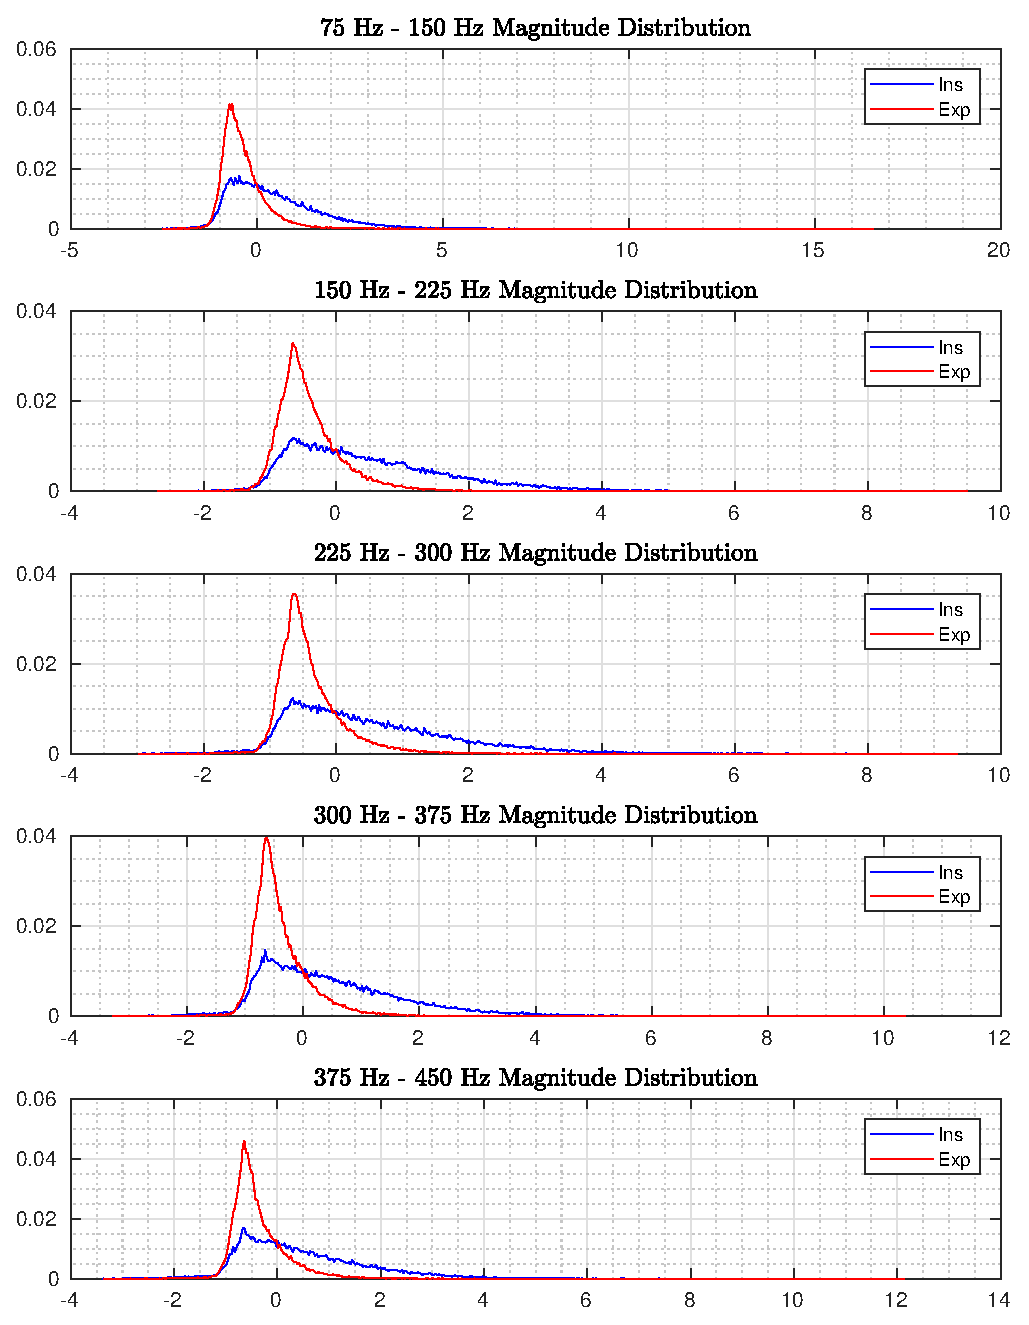
\includegraphics[width=\textwidth]{figures/spectral_ins_exp.eps}
		\caption{Distribution of Spectral Magnitudes For Inspiration and Expiration}
		\label{fig:spectral_ins_exp}
	\end{center}
\end{figure}
\subsubsection{Kurtosis}
Kurtosis is the ratio of the fourth moment to square of second moment. It is a statistical feature which have been used in respiratory signal analysis. Formula for kurtosis is given in \eqref{eq:kurtosis}\\ Distributions of kurtosis of windows during inspiration and expiration for third channel is given in Figure \ref{fig:kurtosis_ins_exp}. 
\begin{equation}\label{eq:kurtosis}
K = |X|\frac{\sum_{x \in X}(x-\hat{\mu}_X)^4}{(\sum_{x \in X}(x-\hat{\mu}_X)^2)^2}
\end{equation}
\begin{figure}
	\begin{center}
		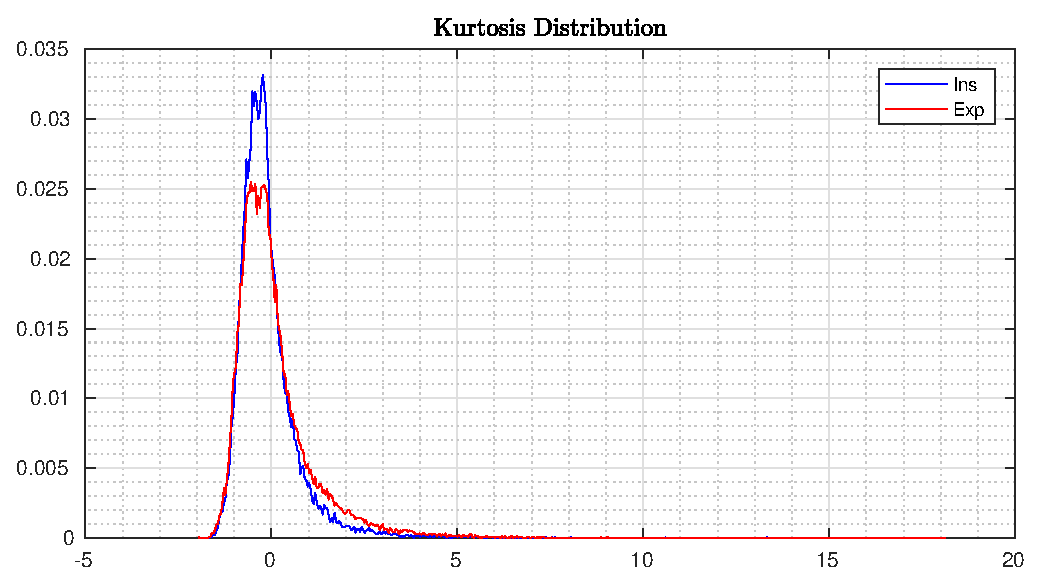
\includegraphics[width=\textwidth]{figures/kurtosis_ins_exp.eps}
		\caption{Distribution of Kurtosis For Inspiration and Expiration}
		\label{fig:kurtosis_ins_exp}
	\end{center}
\end{figure} \par 
The average KL-divergence for features is given in figure \ref{fig:kl_divergence}. The feature indices are consistent with the order features are explained above.
\begin{figure}
	\begin{center}
		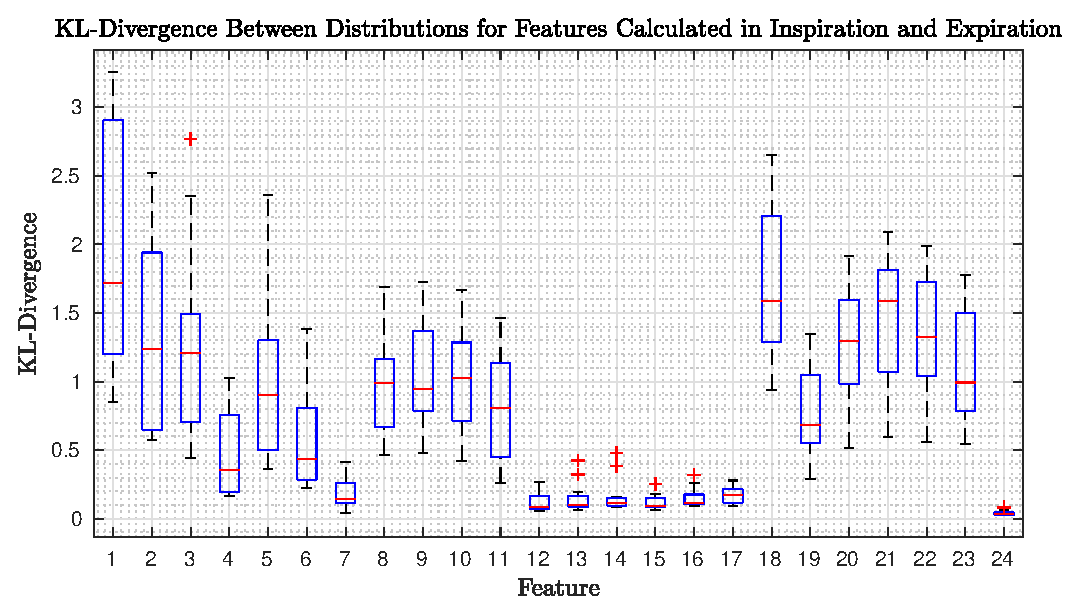
\includegraphics[width=\textwidth]{figures/kl_divergence.eps}
		\caption{KL-Divergence Between Distributions for Features Calculated in Inspiration and Expiration}
		\label{fig:kl_divergence}
	\end{center}
\end{figure} 
\subsection{Denoisining The Output of Neural Network}
The output of neural network is not very good in terms of estimating the phase correctly and it is alternating too much even in short durations. In order to overcome this issue, a filtering was needed. Linear filters don't perform well since they show many discontiunity, so we decided to use a filter that counts the contiunity into account and since we had estimated the period earlier, we tried to use that for filtering purposes. Then we created a periodic square wave with the period equal to the the estimated period and $50\%$ duty cycle. We calculated the cross correlation between this square wave and the output of neural network. This shows us the required amount of shift that is needed for the square wave to fit on to the phase of airflow. We must note that, here we assume that the airflow is periodic and its duty cycle is $50\%$. 